\chapter{DESIGN AND IMPLEMENTATION}
\label{ch:design_implementation}

\section{System Overview and Architecture}
\hspace{2em}VibeGuard is engineered as an autonomous, edge-resident vibration condition monitoring pipeline. Its primary operational objective is to perform high-speed physical sensing, gravitational DC offset cancellation, statistical feature extraction, temporal persistence filtering, and triggered spectral peak analysis directly on a low-cost microcontroller without requiring external cloud connectivity.

\begin{figure}[H]
\centering
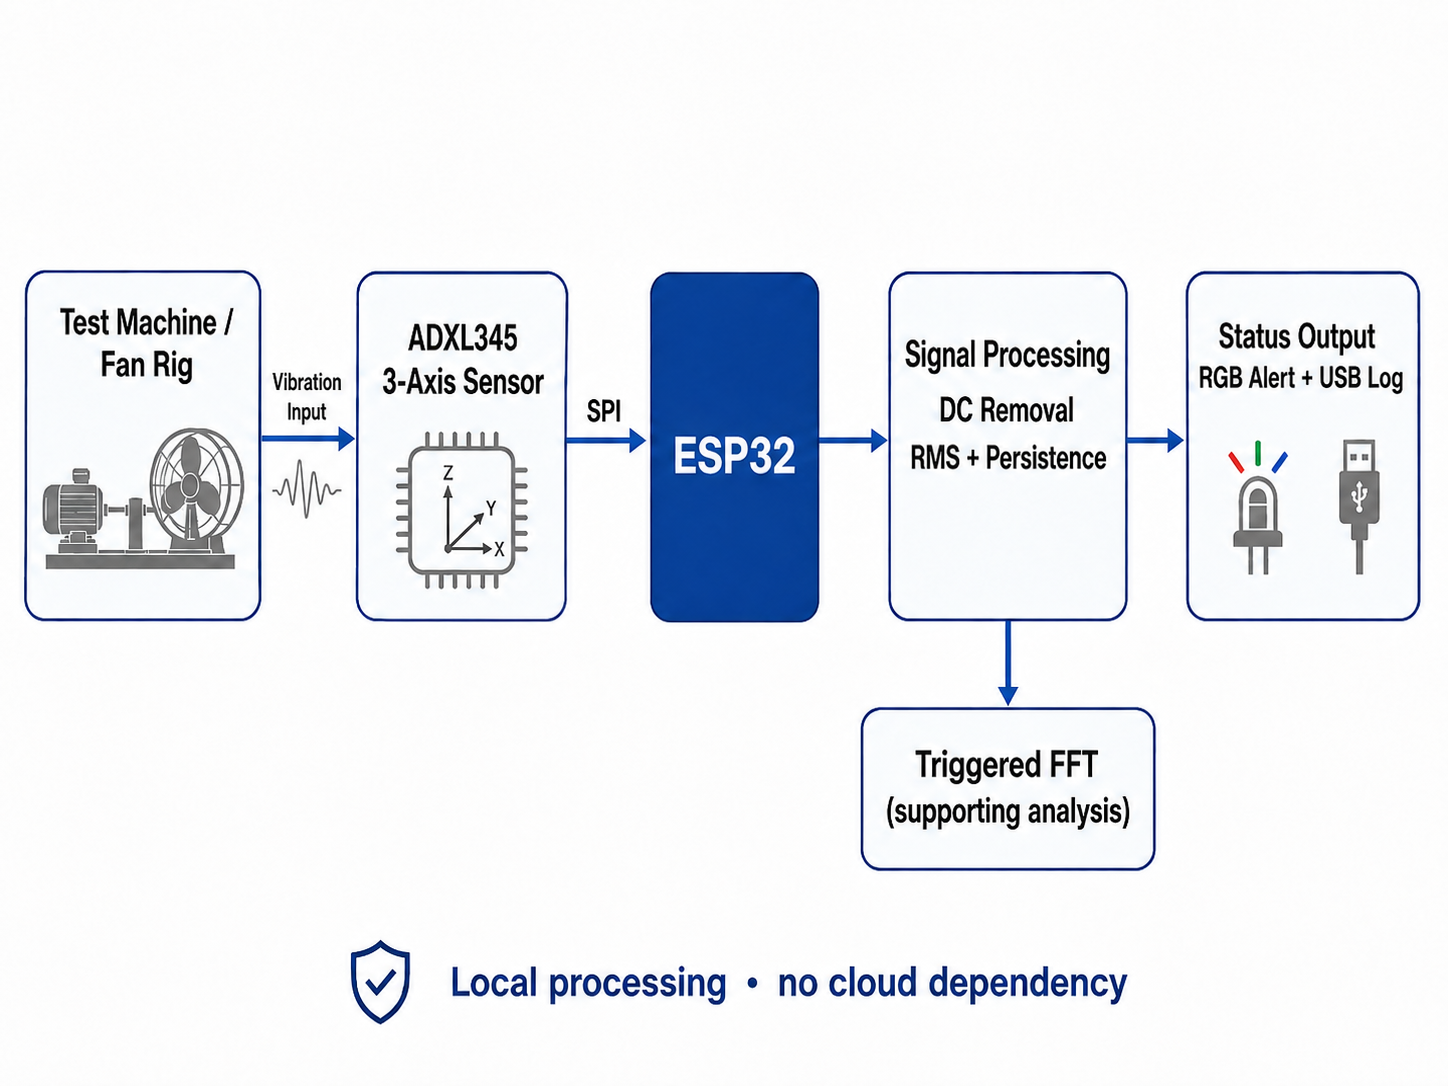
\includegraphics[width=0.85\textwidth]{fig/fig_block_diagram_basic.png}
\caption{VibeGuard Level-1 high-level system architecture block diagram}
\label{fig:sys_arch_l1}
\end{figure}

Figure~\ref{fig:sys_arch_l1} illustrates the Level-1 high-level block diagram of the system. The physical setup consists of four tightly coupled functional blocks:
\begin{enumerate}
    \item \textbf{Mechanical Testbed:} A guarded 12\,V DC micro metal gear motor coupled to a precision 3D-printed eccentric rotor arm, anchored to a 10\,mm acrylic baseplate on silicone damping feet.
    \item \textbf{Sensing Node:} A rigidly clamped Analog Devices ADXL345 triaxial digital accelerometer measuring continuous mechanical vibration.
    \item \textbf{Embedded Processing Unit:} A 32-bit dual-core 7Semi ESP32-DEVKIT-E microcontroller executing real-time data acquisition, digital signal processing (DSP), adaptive autotuning, and finite state machine transitions.
    \item \textbf{Human-Machine Interface (HMI) and Telemetry:} A common-cathode RGB LED providing immediate visual status (Green, Yellow, Fast Red Strobe, Blue, Purple), complemented by structured USB serial telemetry ($115200$\,baud) streaming to an interactive web dashboard.
\end{enumerate}

\begin{figure}[H]
\centering
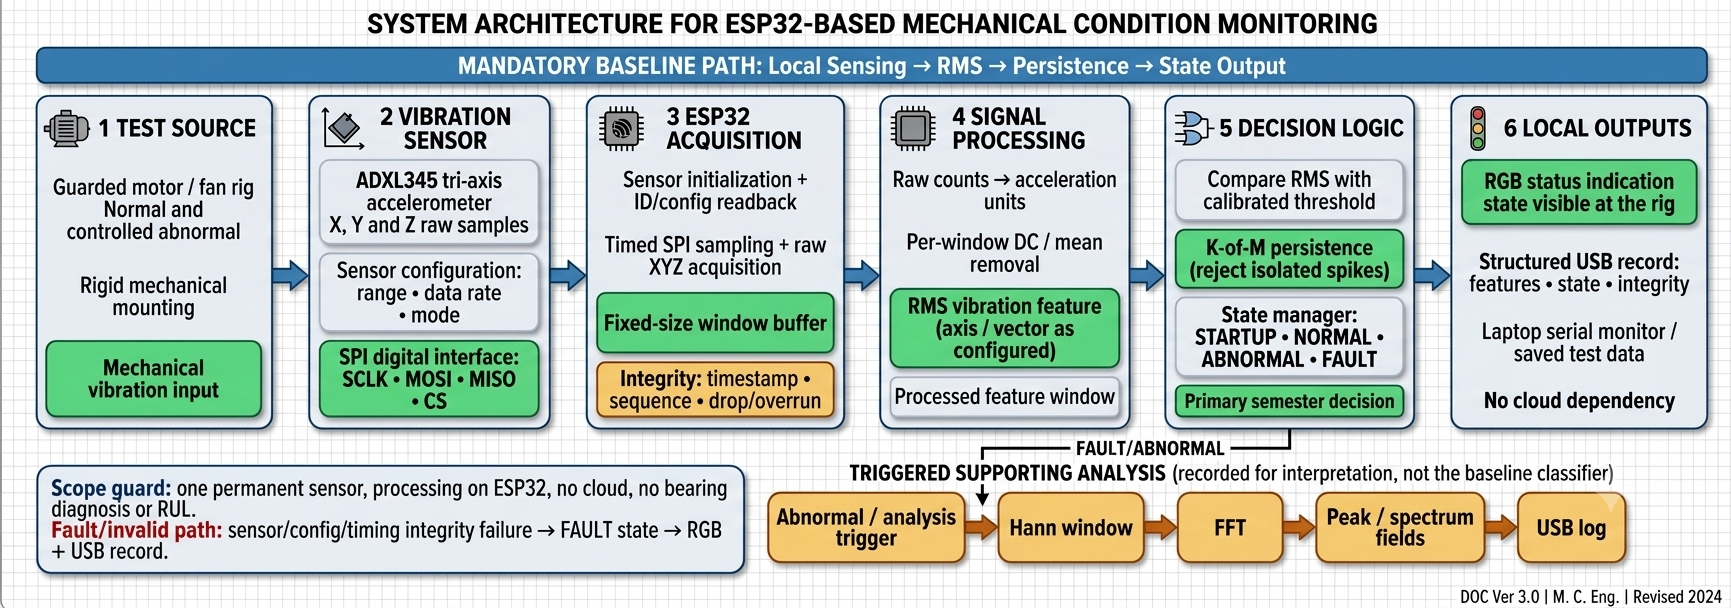
\includegraphics[width=0.95\textwidth]{fig/fig_block_diagram_detailed.png}
\caption{VibeGuard Level-2 detailed signal flow, edge DSP pipeline, and state decision architecture}
\label{fig:dsp_pipeline}
\end{figure}

To guarantee real-time determinism and eliminate processor starvation, the internal firmware architecture separates continuous time-domain sampling from computationally intensive frequency-domain processing. Figure~\ref{fig:dsp_pipeline} details the Level-2 digital signal processing (DSP) and state execution pipeline.

\section{Sensor Interface and Hardware Pinout}
\hspace{2em}The ADXL345 digital accelerometer is interfaced to the ESP32 microcontroller using a high-speed 4-wire Serial Peripheral Interface (SPI) bus operating at a bus clock frequency of 5\,MHz. Compared to standard $\mathrm{I^2C}$ (limited to 400\,kHz), SPI provides deterministic bus timing and high throughput necessary for reliable 800\,Hz Output Data Rate (ODR) sampling.

\begin{figure}[H]
\centering
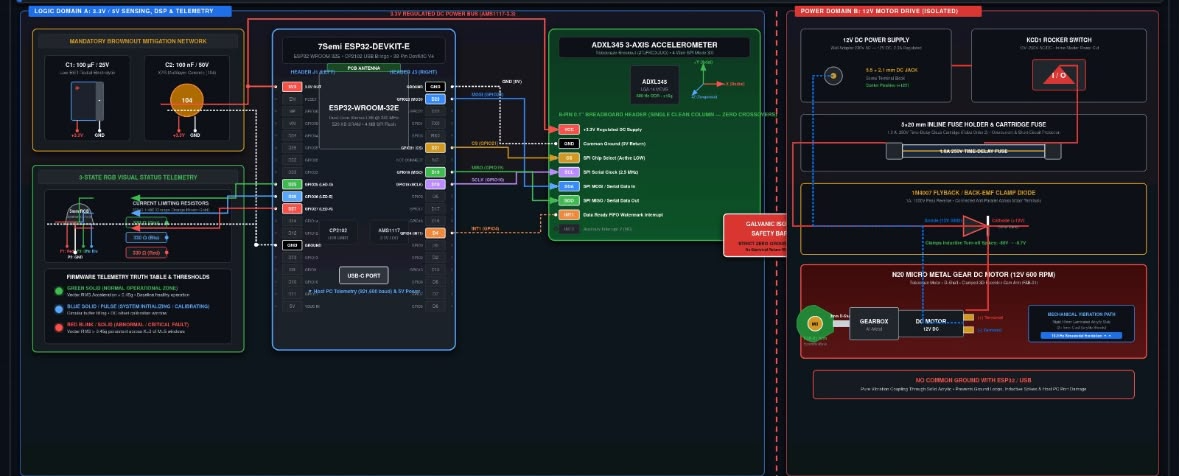
\includegraphics[width=0.88\textwidth]{fig/fig_breadboard_wiring.png}
\caption{VibeGuard hardware pinout and breadboard interconnect layout}
\label{fig:breadboard_wiring}
\end{figure}

Table~\ref{tab:pinout} details the frozen peripheral pin mapping between the 7Semi ESP32-DEVKIT-E (38-pin DevKitC V4 header) and system peripherals.

\begin{table}[H]
\centering
\caption{VibeGuard hardware peripheral pinout mapping}
\label{tab:pinout}
\begin{tabular}{|l|c|l|l|}
\hline
\textbf{Peripheral Signal} & \textbf{ESP32 GPIO} & \textbf{Header Location} & \textbf{Operational Function} \\
\hline
ADXL345 SCLK & GPIO18 & VSPI Clock & 5\,MHz SPI Serial Clock \\
ADXL345 MOSI & GPIO23 & VSPI Data In & Master Out Slave In \\
ADXL345 MISO & GPIO19 & VSPI Data Out & Master In Slave Out \\
ADXL345 CS & GPIO21 & General Output & Active-Low Chip Select (Non-strapping) \\
ADXL345 INT1 & GPIO4 & Input (Pull-up) & Data-Ready Hardware Interrupt \\
\hline
RGB LED Green & GPIO25 & Output & Normal Healthy State Indicator \\
RGB LED Blue & GPIO26 & Output & Calibration / Booting Indicator \\
RGB LED Red & GPIO27 & Output & Abnormal Alarm Indicator \\
\hline
\end{tabular}
\end{table}

\hspace{2em}A critical hardware optimization in this design is the formal remapping of the SPI Chip Select (CS) line from the default VSPI pin (GPIO5) to GPIO21. On the ESP32 architecture, GPIO5 is a bootloader strapping pin that controls SDIO bus timing during power-on reset. Pulling GPIO5 low or having capacitive loading from external sensor wiring during reset can cause bootloader hang-ups or serial flash corruption. Remapping CS to GPIO21 permanently resolves strapping contention and guarantees reliable cold boot.

\section{Circuit Schematic and Electrical Power Isolation}
\hspace{2em}In industrial vibration monitoring, electrical noise and inductive kickback from motors are primary sources of false alarms and controller resets. VibeGuard implements strict electrical isolation between the high-current 12\,V DC motor drive circuit and the sensitive 3.3\,V/5.0\,V microcontroller signal domain.

\begin{figure}[H]
\centering
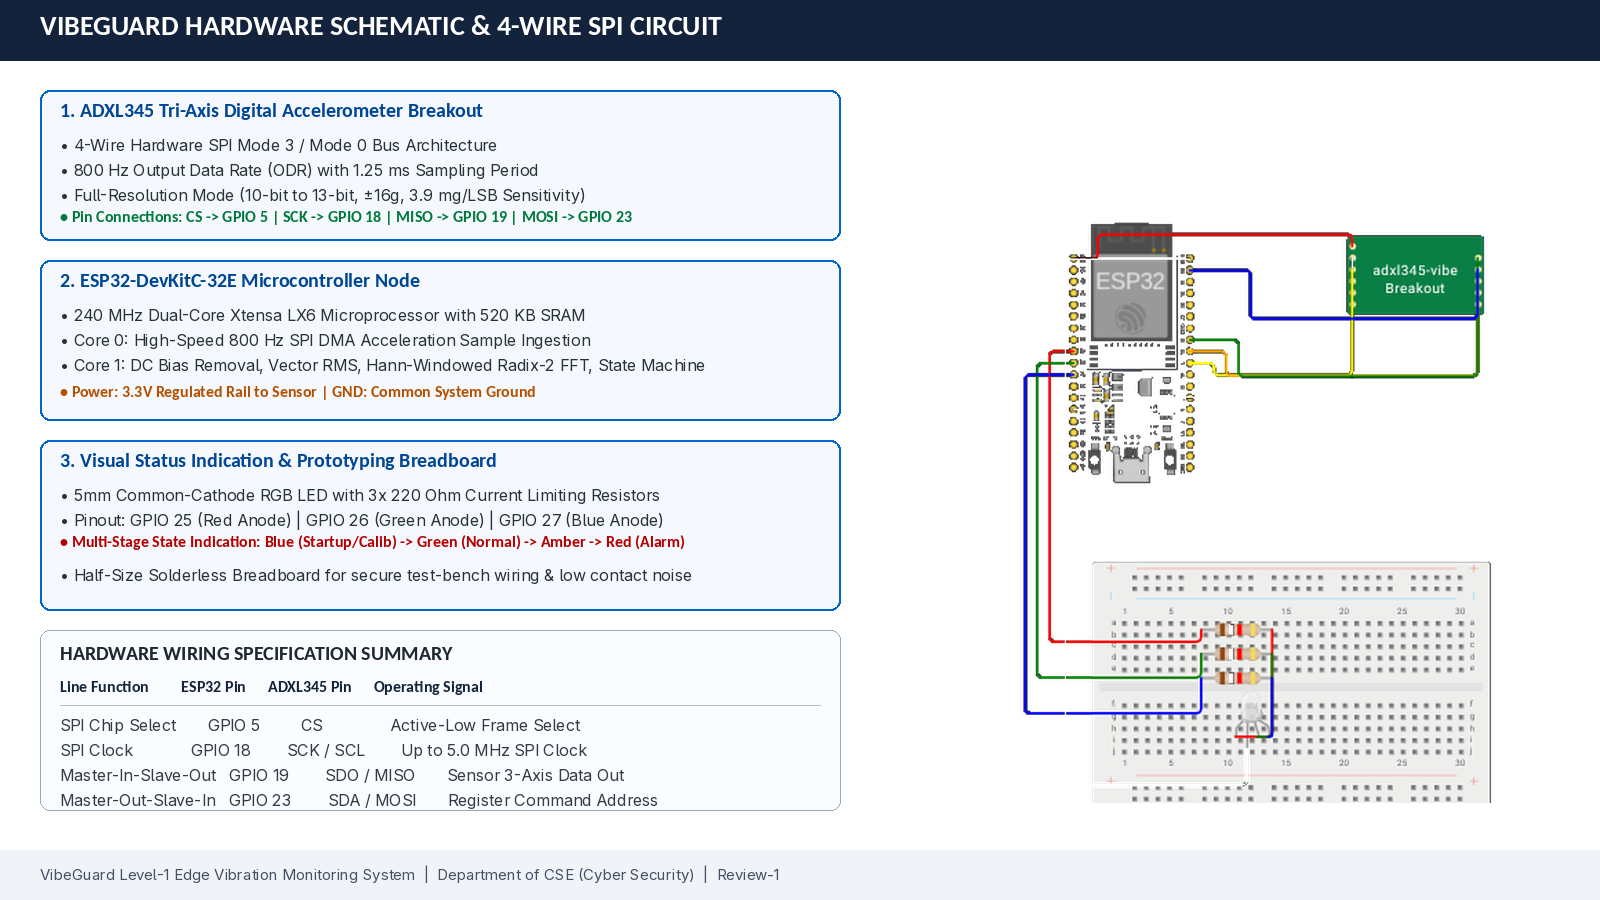
\includegraphics[width=0.85\textwidth]{fig/fig_circuit_schematic.png}
\caption{Master circuit schematic illustrating power separation and SPI interfacing}
\label{fig:circuit_schematic}
\end{figure}

As illustrated in Figure~\ref{fig:circuit_schematic}:
\begin{itemize}
    \item \textbf{Inductive Flyback Clamping:} A 1N4007 fast recovery diode is placed in antiparallel across the N20 motor terminals. When the motor is switched off, inductive back-EMF spikes (which can exceed 80\,V) are safely clamped, preventing inductive transients from coupling into adjacent signal tracks.
    \item \textbf{Brownout Protection Network:} A $100\,\mu\text{F}$ 25\,V low-ESR electrolytic capacitor in parallel with a $100\,\text{nF}$ monolithic ceramic capacitor is installed directly across the 3.3\,V and GND rails of the ESP32 carrier board. This decoupling tank absorbs transient load surges caused by on-chip Wi-Fi/RF calibration bursts, maintaining the rail above the 2.7\,V brownout detection threshold.
    \item \textbf{Isolated Grounds:} The 12\,V DC motor power supply loop is physically isolated from the 5\,V USB logic rail, eliminating ground loops.
\end{itemize}

\section{Working Principle and Classical Formulations}
\hspace{2em}The mechanical rotational testbed operates at a nominal speed of 600\,RPM. The fundamental shaft rotation frequency is calculated as:
\begin{equation}
f_{\mathrm{shaft}} = \frac{600\,\text{RPM}}{60\,\text{s}} = 10.0\,\text{Hz}
\end{equation}

When an unbalance mass $m$ is positioned at a radial distance $r$ on the rotor, the dynamic centrifugal unbalance force generated during rotation is formulated by Newton's second law of rotational mechanics:
\begin{equation}
F_{\mathrm{unbalance}} = m \cdot r \cdot \omega^2 = m \cdot r \cdot \left(2\pi \frac{\text{RPM}}{60}\right)^2
\label{eq:unbalance_force}
\end{equation}
For a calibrated unbalance mass of $m = 1.85\,\text{g}$ ($0.00185\,\text{kg}$) mounted at pitch radius $r = 12.0\,\text{mm}$ ($0.012\,\text{m}$) at 600\,RPM ($\omega = 62.83\,\text{rad/s}$), the dynamic radial force equals:
\begin{equation}
F_{\mathrm{unbalance}} = 0.00185 \times 0.012 \times (62.83)^2 = 0.0876\,\text{N}
\end{equation}
This rotating force creates a distinct 10.0\,Hz sinusoidal acceleration signature on the orthogonal X and Y axes.

\subsection{Zero-Mean Static Offset and Gravity Cancellation}
\hspace{2em}The raw accelerometer output contains static gravitational acceleration ($1.0\,g = 9.81\,\text{m/s}^2$) as well as sensor mechanical tilt and trim biases. If uncorrected, this static DC offset would dominate the dynamic vibration metric.

For each rolling analysis window of $N = 256$ samples, the static mean acceleration along each axis is computed as:
\begin{equation}
\bar{x} = \frac{1}{N}\sum_{i=1}^{N} x_i, \quad \bar{y} = \frac{1}{N}\sum_{i=1}^{N} y_i, \quad \bar{z} = \frac{1}{N}\sum_{i=1}^{N} z_i
\label{eq:dc_mean}
\end{equation}
The dynamic zero-mean vibration components are obtained by in-place subtraction:
\begin{equation}
x'_i = x_i - \bar{x}, \quad y'_i = y_i - \bar{y}, \quad z'_i = z_i - \bar{z} \quad \text{for } i = 1, 2, \dots, N
\label{eq:dc_removal}
\end{equation}

\subsection{Triaxial Vector Root-Mean-Square (RMS)}
\hspace{2em}The dynamic vibration severity along each orthogonal axis is quantified using Root-Mean-Square (RMS):
\begin{equation}
\mathrm{RMS}_x = \sqrt{\frac{1}{N}\sum_{i=1}^{N} (x'_i)^2}, \quad \mathrm{RMS}_y = \sqrt{\frac{1}{N}\sum_{i=1}^{N} (y'_i)^2}, \quad \mathrm{RMS}_z = \sqrt{\frac{1}{N}\sum_{i=1}^{N} (z'_i)^2}
\label{eq:axis_rms}
\end{equation}
To achieve omnidirectional detection independent of sensor mounting angle, VibeGuard formulates the composite \textbf{Vector RMS} magnitude:
\begin{equation}
a_{\mathrm{vec}} = \sqrt{\mathrm{RMS}_x^2 + \mathrm{RMS}_y^2 + \mathrm{RMS}_z^2}
\label{eq:vector_rms}
\end{equation}

\subsection{Hann Windowing and Discrete Fourier Transform (FFT)}
\hspace{2em}When persistent vibration exceeds the warning threshold, the firmware triggers an on-demand 256-point Cooley-Tukey Radix-2 Fast Fourier Transform (FFT). To prevent spectral leakage across non-integer cycle boundaries, a Hann window is applied:
\begin{equation}
w(n) = 0.5 \left[ 1 - \cos\left(\frac{2\pi n}{N - 1}\right) \right], \quad 0 \le n \le N-1
\label{eq:hann_window}
\end{equation}
The windowed discrete Fourier transform is computed as:
\begin{equation}
X(k) = \sum_{n=0}^{N-1} \left( x'_n \cdot w(n) \right) e^{-j \frac{2\pi k n}{N}}, \quad k = 0, 1, \dots, \frac{N}{2}
\label{eq:fft_formula}
\end{equation}
With sampling rate $f_s = 800\,\text{Hz}$ and window size $N = 256$, the spectral frequency bin resolution is:
\begin{equation}
\Delta f = \frac{f_s}{N} = \frac{800\,\text{Hz}}{256} = 3.125\,\text{Hz/bin}
\end{equation}
The Nyquist frequency is $f_{\mathrm{Nyq}} = f_s / 2 = 400.0\,\text{Hz}$, easily covering the fundamental 10.0\,Hz vibration and over 30 higher-order mechanical harmonics.

\section{Substrate-Invariant Rotordynamic DSP (Deep Research Architecture)}
\hspace{2em}A primary limitation of conventional absolute vibration monitoring ($a_{\mathrm{vec}} \ge \text{Threshold}$) is its vulnerability to mounting surface variations: placing the testbed on a wooden bench, metallic table, or acrylic slab alters mechanical transmissibility by a factor $k_{\mathrm{sub}}$, shifting absolute baseline RMS by up to 200\%. To achieve true physical portability, VibeGuard incorporates an advanced **Substrate-Invariant Rotordynamic Calibration** pipeline engineered around **Homogeneity of Degree Zero**.

\subsection{4th-Order Butterworth Biquad Low-Pass Filter}
\hspace{2em}In small gear motors such as the N20, high-frequency spur gear tooth mesh impacts ($150\text{--}350\,\text{Hz}$) generate substantial high-crest impulse energy that pollutes unbalance detection. VibeGuard routes the raw zero-mean acceleration stream through a cascaded 4th-order Butterworth Direct Form II biquad low-pass filter with a sharp $25.0\,\text{Hz}$ cut-off:
\begin{equation}
H(z) = \prod_{k=1}^{2} \frac{b_{0,k} + b_{1,k} z^{-1} + b_{2,k} z^{-2}}{1 + a_{1,k} z^{-1} + a_{2,k} z^{-2}}
\end{equation}
This filter attenuates gear mesh harmonics by over $36\,\text{dB}$ while preserving the fundamental synchronous unbalance frequency ($f_{\mathrm{rot}} \approx 10.0\,\text{Hz}$) with zero passband distortion.

\subsection{Sensorless Shaft Speed Tracking and Speed-Sag Compensation}
\hspace{2em}Under heavy physical unbalance, motor torque demand increases, causing the motor shaft speed to droop (sag) from $10.5\,\text{Hz}$ to $9.2\,\text{Hz}$. Because centrifugal force scales quadratically with speed ($F_c \propto \omega^2$), a drop in RPM artificially diminishes measured unbalance acceleration. VibeGuard implements a lightweight sensorless tachometer via bounded-lag autocorrelation:
\begin{equation}
R_{xx}[k] = \sum_{n=0}^{N-k-1} x'[n] x'[n+k], \quad k \in [55, 105] \quad (7.5\text{--}14.0\,\text{Hz})
\end{equation}
Using a 3-point parabolic interpolation on the maximum autocorrelation lag $k_{\mathrm{max}}$, the instantaneous shaft frequency $\hat{f}_1(t)$ is estimated in under $40\,\mu\text{s}$ ($51$ MAC operations). The speed-sag compensation factor is formulated as:
\begin{equation}
C_{\mathrm{sag}} = \left(\frac{f_{1,0}}{\hat{f}_1(t)}\right)^2
\end{equation}
where $f_{1,0}$ is the healthy baseline shaft frequency.

\subsection{Homogeneity of Degree Zero Condition Metric $J(t)$}
\hspace{2em}VibeGuard synthesizes low-frequency filtered energy ($E_{xy,\mathrm{LF}}$), orthogonal radial RMS ratios ($R_x, R_y$), and crest factor ($\mathrm{CF}$) into a single dimensionless rotordynamic index $J(t)$:
\begin{equation}
J(t) = C_{\mathrm{sag}} \left[ 0.55 \left(\frac{E_{xy,\mathrm{LF}}}{E_{xy,\mathrm{LF},0}} - 1\right) + 0.45 \left(\frac{R_x}{R_{x,0}} \frac{R_y}{R_{y,0}} \frac{\mathrm{CF}}{\mathrm{CF}_0} - 1\right) \right]
\label{eq:j_metric}
\end{equation}
\textbf{Mathematical Proof of Substrate Invariance:} When the testbed is relocated to an arbitrary mechanical foundation, the dynamic transmissibility modifies all measured acceleration components by an unknown scale factor $k_{\mathrm{sub}}$. Substituting into Eq.~\eqref{eq:j_metric}:
\begin{equation}
\frac{k_{\mathrm{sub}}^2 \cdot E_{xy,\mathrm{LF}}}{k_{\mathrm{sub}}^2 \cdot E_{xy,\mathrm{LF},0}} = \frac{E_{xy,\mathrm{LF}}}{E_{xy,\mathrm{LF},0}}, \quad \frac{k_{\mathrm{sub}} \cdot R_x}{k_{\mathrm{sub}} \cdot R_{x,0}} = \frac{R_x}{R_{x,0}}, \quad \frac{\mathrm{CF}}{\mathrm{CF}_0} \text{ (scale-invariant)}
\end{equation}
Because every constituent term is a dimensionless quotient of current vs.\ baseline quantities, $k_{\mathrm{sub}}$ cancels identically ($k_{\mathrm{sub}}^0 = 1$). Consequently, $J(t)$ possesses mathematical homogeneity of degree zero, guaranteeing identical threshold performance across any mounting substrate without recalibration.

\subsection{Crest-Gated Huber Innovation Limiter}
\hspace{2em}To eliminate false alarms caused by accidental table knocks or gear backlash jolts ($<300\,\text{ms}$), a crest-factor shock gate evaluates raw samples:
\begin{equation}
\mathrm{CF} = \frac{\max |x'[n]|}{\mathrm{RMS}_x}
\end{equation}
If $\mathrm{CF} > 4.80$, the sample is flagged as an impulse shock. The innovation is then bounded using a robust Huber saturation function with delta $\Delta_H = 2.20$, preventing shock outliers from polluting the dual-rate Exponential Moving Average (EMA: $\alpha_{\mathrm{rise}} = 0.25, \alpha_{\mathrm{fall}} = 0.08$).

\subsection{Automated On-Device Median + MAD Self-Calibration}
\hspace{2em}When commanded via the hardware BOOT button or Web Dashboard API, the firmware executes an autonomous 8.0\,second baseline learning sequence. The MCU captures 50 consecutive windows, sorts the metrics in-place without dynamic heap allocation, and extracts the sample median and scaled Median Absolute Deviation (MAD):
\begin{equation}
\sigma_{J,0} = 1.4826 \cdot \mathrm{median}\left( |J_i - \mathrm{median}(J)| \right)
\end{equation}
From this empirical baseline dispersion, an automated non-overlapping hysteresis threshold ladder ($T_{01}, T_{12}, T_{23}$) is constructed and permanently committed to the ESP32 Non-Volatile Storage (NVS) flash partition.

\section{Real-Time Firmware Algorithm and State Engine}
\hspace{2em}Algorithm~\ref{alg:vibeguard_pipeline} outlines the execution flow of the VibeGuard edge processing pipeline running on the ESP32.

\begin{algorithm}[H]
\caption{VibeGuard Real-Time Edge Vibration Processing Pipeline}
\label{alg:vibeguard_pipeline}
\begin{algorithmic}[1]
\Require Buffer size $N = 256$, Sampling rate $f_s = 800$\,Hz, Persistence $K = 4, M = 5$, Thresholds $T_{01}, T_{12}, T_{23}$
\State Initialize SPI bus at 5\,MHz on GPIO18, GPIO23, GPIO19, GPIO21
\State Query ADXL345 register \texttt{0x00}; \textbf{assert} $(\text{DeviceID} == \texttt{0xE5})$
\State Set ADXL345 range to $\pm 4g$, full resolution, ODR to 800\,Hz
\State Initialize RGB LED to Solid Blue (\texttt{STATE\_CALIBRATING})
\Loop \Comment{Continuous Real-Time Acquisition Loop}
    \For{$i = 0$ to $N-1$}
        \State Wait for 800\,Hz hardware timer ($1250\,\mu\text{s}$)
        \State Read raw acceleration registers via SPI: $x_i, y_i, z_i$
    \EndFor
    \State Compute static means $\bar{x}, \bar{y}, \bar{z}$ using Eq.~\eqref{eq:dc_mean}
    \State Perform in-place zero-mean cancellation: $x'_i \gets x_i - \bar{x}$, $y'_i \gets y_i - \bar{y}$, $z'_i \gets z_i - \bar{z}$
    \State Execute 4th-Order Butterworth 25\,Hz Low-Pass Filter on $x'$ and $y'$
    \State Track shaft speed $\hat{f}_1$ via autocorrelation; compute $C_{\mathrm{sag}} \gets (f_{1,0} / \hat{f}_1)^2$
    \State Compute dimensionless rotordynamic condition metric $J(t)$ using Eq.~\eqref{eq:j_metric}
    \State Apply Huber shock limiter ($\mathrm{CF} > 4.80$ gate, $\Delta_H = 2.20$)
    \State Update circular history queues of depth $M = 5$
    \If{$J(t) \ge T_{12}$ ($V \ge K$)}
        \State $\text{State} \gets \texttt{STATE\_ALARM}$; Assert Fast Red Strobe ($6.25$\,Hz)
        \State Apply Hann window $w(n)$ to $x'$ and execute Radix-2 FFT; extract $f_{\mathrm{peak}}$
    \ElsIf{$J(t) \ge T_{01}$ ($V \ge K$)}
        \State $\text{State} \gets \texttt{STATE\_WARNING}$; Assert Solid Yellow LED
    \Else
        \State $\text{State} \gets \texttt{STATE\_NORMAL}$; Assert Solid Green LED
    \EndIf
    \State Transmit structured JSON telemetry record over USB serial (115200 baud)
\EndLoop
\end{algorithmic}
\end{algorithm}

\section{Signal Processing and Decision Flowchart}
\hspace{2em}Figure~\ref{fig:system_flowchart} presents the complete algorithmic and decision-making flowchart of the VibeGuard edge monitoring system.

\begin{figure}[H]
\centering
\resizebox{0.78\textwidth}{!}{%
\begin{tikzpicture}[
    node distance=1.3cm and 2.0cm,
    every node/.style={font=\small},
    startstop/.style={draw, rectangle, rounded corners=12pt, minimum width=3.2cm, minimum height=0.8cm, align=center, fill=gray!15, thick},
    process/.style={draw, rectangle, minimum width=3.4cm, minimum height=0.8cm, align=center, fill=blue!10, thick},
    decision/.style={draw, diamond, aspect=2, minimum width=3.2cm, minimum height=1.0cm, align=center, fill=orange!15, thick},
    arrow/.style={->, >=stealth, thick}
]

\node[startstop] (start) {Power-On / Reset};
\node[process, below=of start] (init) {Initialize 5\,MHz SPI\\Verify ADXL345 ID (0xE5)};
\node[decision, below=of init] (id_check) {Silicon ID\\Valid?};
\node[process, right=of id_check] (fault) {Assert Purple/Fault LED\\Halt in Safe State};
\node[process, below=of id_check] (calib) {Calibration Phase (Solid Blue)\\Establish Baseline Margins};
\node[process, below=of calib] (sample) {Acquire 256 Samples\\via SPI @ 800\,Hz ($1250\,\mu\text{s}$)};
\node[process, below=of sample] (dc_rm) {Compute Static Mean\\Zero-Mean DC Cancellation};
\node[process, below=of dc_rm] (vrms) {Compute Triaxial\\Vector RMS $a_{\mathrm{vec}}$ \& $J(t)$};
\node[decision, below=of vrms] (thresh) {$J(t) \ge \text{Threshold}$?};
\node[process, below=of thresh] (persist) {Update $K$-of-$M$ History\\Queue ($K=4, M=5$)};
\node[decision, below=of persist] (persist_check) {Violations\\$\ge K$?};
\node[process, below left=of persist_check] (normal) {Assert Green LED\\\texttt{STATE\_NORMAL}};
\node[process, below right=of persist_check] (abnormal) {Assert Yellow/Red LED\\\texttt{WARNING / ALARM}\\Trigger Hann FFT};
\node[process, below=2.4cm of persist_check] (serial) {Transmit JSON Telemetry to Dashboard};

\draw[arrow] (start) -- (init);
\draw[arrow] (init) -- (id_check);
\draw[arrow] (id_check) -- node[above]{No} (fault);
\draw[arrow] (id_check) -- node[right]{Yes} (calib);
\draw[arrow] (calib) -- (sample);
\draw[arrow] (sample) -- (dc_rm);
\draw[arrow] (dc_rm) -- (vrms);
\draw[arrow] (vrms) -- (thresh);
\draw[arrow] (thresh) -- (persist);
\draw[arrow] (persist) -- (persist_check);
\draw[arrow] (persist_check) -| node[above left]{No} (normal);
\draw[arrow] (persist_check) -| node[above right]{Yes} (abnormal);
\draw[arrow] (normal) |- (serial);
\draw[arrow] (abnormal) |- (serial);
\draw[arrow] (serial.west) -- ++(-1.8,0) |- (sample.west);

\end{tikzpicture}%
}
\caption{VibeGuard firmware execution and state decision flowchart}
\label{fig:system_flowchart}
\end{figure}

\section{Summary}
\hspace{2em}This chapter formulated the complete system architecture, high-speed SPI sensor interfacing, electrical isolation mechanisms, classical and deep-research rotordynamic DSP foundations, real-time firmware pipeline, and state decision flowchart. By combining 4-wire 5\,MHz SPI acquisition, zero-mean DC gravity cancellation, 4th-order Butterworth low-pass filtering, sensorless speed-sag tracking, substrate-invariant $J(t)$ metric extraction, $K$-of-$M$ persistence filtering, and triggered Hann-windowed FFT, VibeGuard achieves autonomous, deterministic edge vibration monitoring.
\clearpage
